\documentclass[oneside]{article}
\usepackage[latin1]{inputenc}
\usepackage[brazil]{babel}
\usepackage{graphicx}
\usepackage{listings}
\usepackage{xcolor}
\usepackage{amsmath}
\usepackage{hyperref}
\usepackage{url}
\usepackage{breakurl}
\usepackage[left=2.7cm, right=2.7cm, bottom=3cm]{geometry}
\usepackage{caption}
\usepackage{subcaption}
\usepackage{lipsum}
\usepackage{fancyhdr}
\usepackage{listing}
\usepackage{gensymb}
\usepackage{caption}

%\renewcommand*{\refname}{Refer�ncias Bibliogr�ficas}

\fancyfoot[c]{\thepage}
\fancyhead[ro,le]{}
\fancyhead[lo]{\leftmark}
\fancyhead[re]{\rightmark}

\lstset{%
	linewidth=\textwidth,%framed box is the text size 
	xleftmargin=.25in,
	xrightmargin=.25in, 
	frame=trbl, 
	columns=flexible, 
	captionpos=t, 
	upquote=false,
	basicstyle=\small\ttfamily,
	firstnumber=1,% 
	numberfirstline=false,% 
	numbers=left,%
	numberstyle=\tiny,% 
	stepnumber=5,%
	numbersep=5pt,% 
	backgroundcolor=\color{green!15},% 
	tabsize=4,% 
	keywordstyle=\color{green!65!black},% 
	commentstyle=\color{blue},% 
	stringstyle=\color{magenta},% 
	breaklines=true,% 
	emph={label},%
	abovecaptionskip=10pt,% 
	belowcaptionskip={\abovecaptionskip},%
	showstringspaces=false, 
	literate={�}{{\^{E}}}1
}%

\lstdefinestyle{code} {%
	basicstyle=\ttfamily\footnotesize,
	backgroundcolor=\color{blue!10},
	%escapeinside={@}{@},
	frame=single, 
	captionpos=t,
	upquote=false,
	numberfirstline=false,% 
	stepnumber=5,%
	tabsize=4,% 
	keywordstyle=\color{green!65!black},% 
	commentstyle=\color{blue},%
	stringstyle=\color{magenta},% 
	breaklines=true,% 
	emph={label},%
	abovecaptionskip=10pt,% 
	belowcaptionskip={\abovecaptionskip},%
}%

\title{\huge
	\vspace{40pt}
	Sistema de Banco de Dados de uma Escola
	\vspace{25pt}
}

\author{
	Gabriel Peixoto de Carvalho\\
	\texttt{gaburiero.c@gmail.com}\\
	\texttt{201106840010}
	\and
	Thiago Barros Coelho\\
	\texttt{tbarroscoelho@gmail.com}\\
	\texttt{201106840041}
}
\date{
\vspace{100pt}
\begin{table}[!h]
	\begin{tabular*}{.9\linewidth}{p{.45\linewidth}p{.45\linewidth}}
	& Projeto apresentado � disciplina Banco de Dados 
	como requisito de avalia��o.
	Professor: Eloi Favero.
	\end{tabular*}
\end{table}
\vfill
Bel�m -- Brasil\\
\vspace{2pt}
Julho/2015
}

\begin{document}
% capa ------------------------------------------------------------------------
\thispagestyle{empty}
\begin{center}

\includegraphics[width=.16\textwidth]{Figures/logo_ufpa}\\

\vspace{12pt}
\bf\large
UNIVERSIDADE FEDERAL DO PAR�\\\vspace{1.5pt}
INSTITUTO DE TECNOLOGIA\\\vspace{1pt}
FACULDADE DE ENGENHARIA DA COMPUTA��O E\\\vspace{1.5pt}
TELECOMUNICA��ES\\

\vspace{120pt}
{\Large
Sistema de Banco de Dados de uma Escola
}

\vfill
\normalsize
Bel�m -- Brasil\\
Junho/2015
\end{center}
%%% EOF %%%u


% T�tulo e Pre�mbulo -----------------------------------------------------------
\newpage
\maketitle
\thispagestyle{empty}

% Sum�rio e Lista de Figuras ---------------------------------------------------
\newpage
\tableofcontents
\listoffigures

% Introdu��o enunciado da questao-------------------------------------------------------------------
\newpage
\pagestyle{fancy}
\begin{section}{Enunciado da Quest�o}
\textbf{Para o enunciado abaixo:}\\ 
\textbf{(a)} fa�a um modelo conceitual baseado na abordagem Entidade e Relacionamentos
(E-R);  (feito a m�o entregar no dia)... \\
\textbf{(b)} desenhe no dB-designer com todos os campos e gere o esquema do BD (entregar
o esquema textual e diagrama E-R impresso). \\ 
\textbf{(c)} Crie um script para criar o BD no (Interbase ou MySQl...) e um script para
dar carga  com pelo menos 40 alunos/respons�veis 5 professores e duas turmas. E
fa�a todas as consultas em SQL (R1 at� R6), mostrando a sa�da.\\

Considere uma escola de ensino fundamental. Nesta escola desejam-se informatizar
diversos procedimentos, sendo coletados os requisitos que seguem. Primeiro �
necess�rio um cadastro de pais (ou respons�veis). Cada aluno tem um respons�vel
(um dos pais, ou outra pessoa). Para o respons�vel � necess�rio ter ID, nome e
fone.  Todo respons�vel tem um endere�o (string20 e.g. "rua pio X, nro13").\\
Cada matr�cula de um aluno vale para o ano corrente. Para o aluno guarda-se o
nome e fone. Para cada aluno cria-se um ID (inteiro) que vale para todos os anos
que o aluno permanecer no col�gio. Al�m disso, anualmente, cada aluno recebe um
n�mero de matricula composto por (ano, s�rie, turma, n�mero seq��ncia). Exemplos
de n�meros de matricula 20083TA23, 20061TB05. Numa turma s�o aceitos no m�ximo
50 alunos.\\

S�o registrados os valores das provas bimestrais dos alunos (duas vezes por
semestre), por mat�ria (portugu�s, matem�tica, geografia, etc). Se o aluno tirar
nota inferior a 60 fica em recupera��o no final de cada semestre, recebendo a
nota da recupera��o, que substitui a menor nota dos dois bimestres. Devem ser
mantidos registros de todas as provas e recupera��es todas notas de uma mat�ria
s�o registradas nos campos (B1,B2,B3,B4,R1,R2: numeric(2)) para cada
matricula.\\

O sistema deve emitir folhas de freq��ncia (Rel 1), com nome do professor de
cada turma e dos alunos, e da identifica��o da sala (ex. S10, S15); emitir 3
relat�rios.  O sistema deve emitir os boletins de notas (Rel 2) bimestrais
(cumulativo para o ano) para cada aluno; emitir relat�rio de notas para 3
alunos; mostram-se as notas das provas, recupera��es e m�dias semestrais e
anuais. O sistema deve emitir um hist�rico cumulativo (Rel 3) para cada aluno
considerando os v�rios anos; emitir 3 hist�ricos.\\

Para os professores registram-se � necess�rio ter ID, nome e fone. S�o criados
relat�rios com os totais (quantidade) de alunos de recupera��o de cada turma
(Rel 4), com objetivo de prover orienta��o pedag�gica para os alunos com pais.\\

O sistema tamb�m controla o pagamento da mensalidade de cada aluno. S�o emitidos
boletos (Rel 5), com o endere�o do respons�vel; Emitir 2 boletos, com repons�vel
e endere�o e aluno. Para cada aluno devem ser registrados os valores mensais
pagos; s�o registrados para cada ano os valores na base como (valorMens,
m1,m2,m3,m4,...m12:float); meses s�o inicializados zerados, quando pagos
marca-se o valor pago; o vencimento � o dia 7 de cada m�s; � preciso registar a
data do pagto. No momento da matricula � definido o valor a ser pago (valorMens)
que pode ser reajustado durante o ano (somente o valor atual � registrado em
valorMens). A qualquer momento o respons�vel pode solicitar um "extrato" dos
valores pagos e/ou vencidos de um aluno, dentro de um ano (Rel 6); emitir o
comprovante de tr�s alunos. 

\end{section}
%https://en.wikipedia.org/wiki/Turing_machine
%https://pt.wikipedia.org/wiki/Hist�ria_da_computa��o
%%% EOF %%%


% Esquemas e scripts de cria��o e insercao no banco ------------------------------
\begin{section}{Metodologia}

\subsection{Modelo do Banco}
O modelo do banco foi mostrado em aula de laborat�rio pelo professor da
disciplina e segue abaixo.

\begin{figure}[!h]
    \centering
    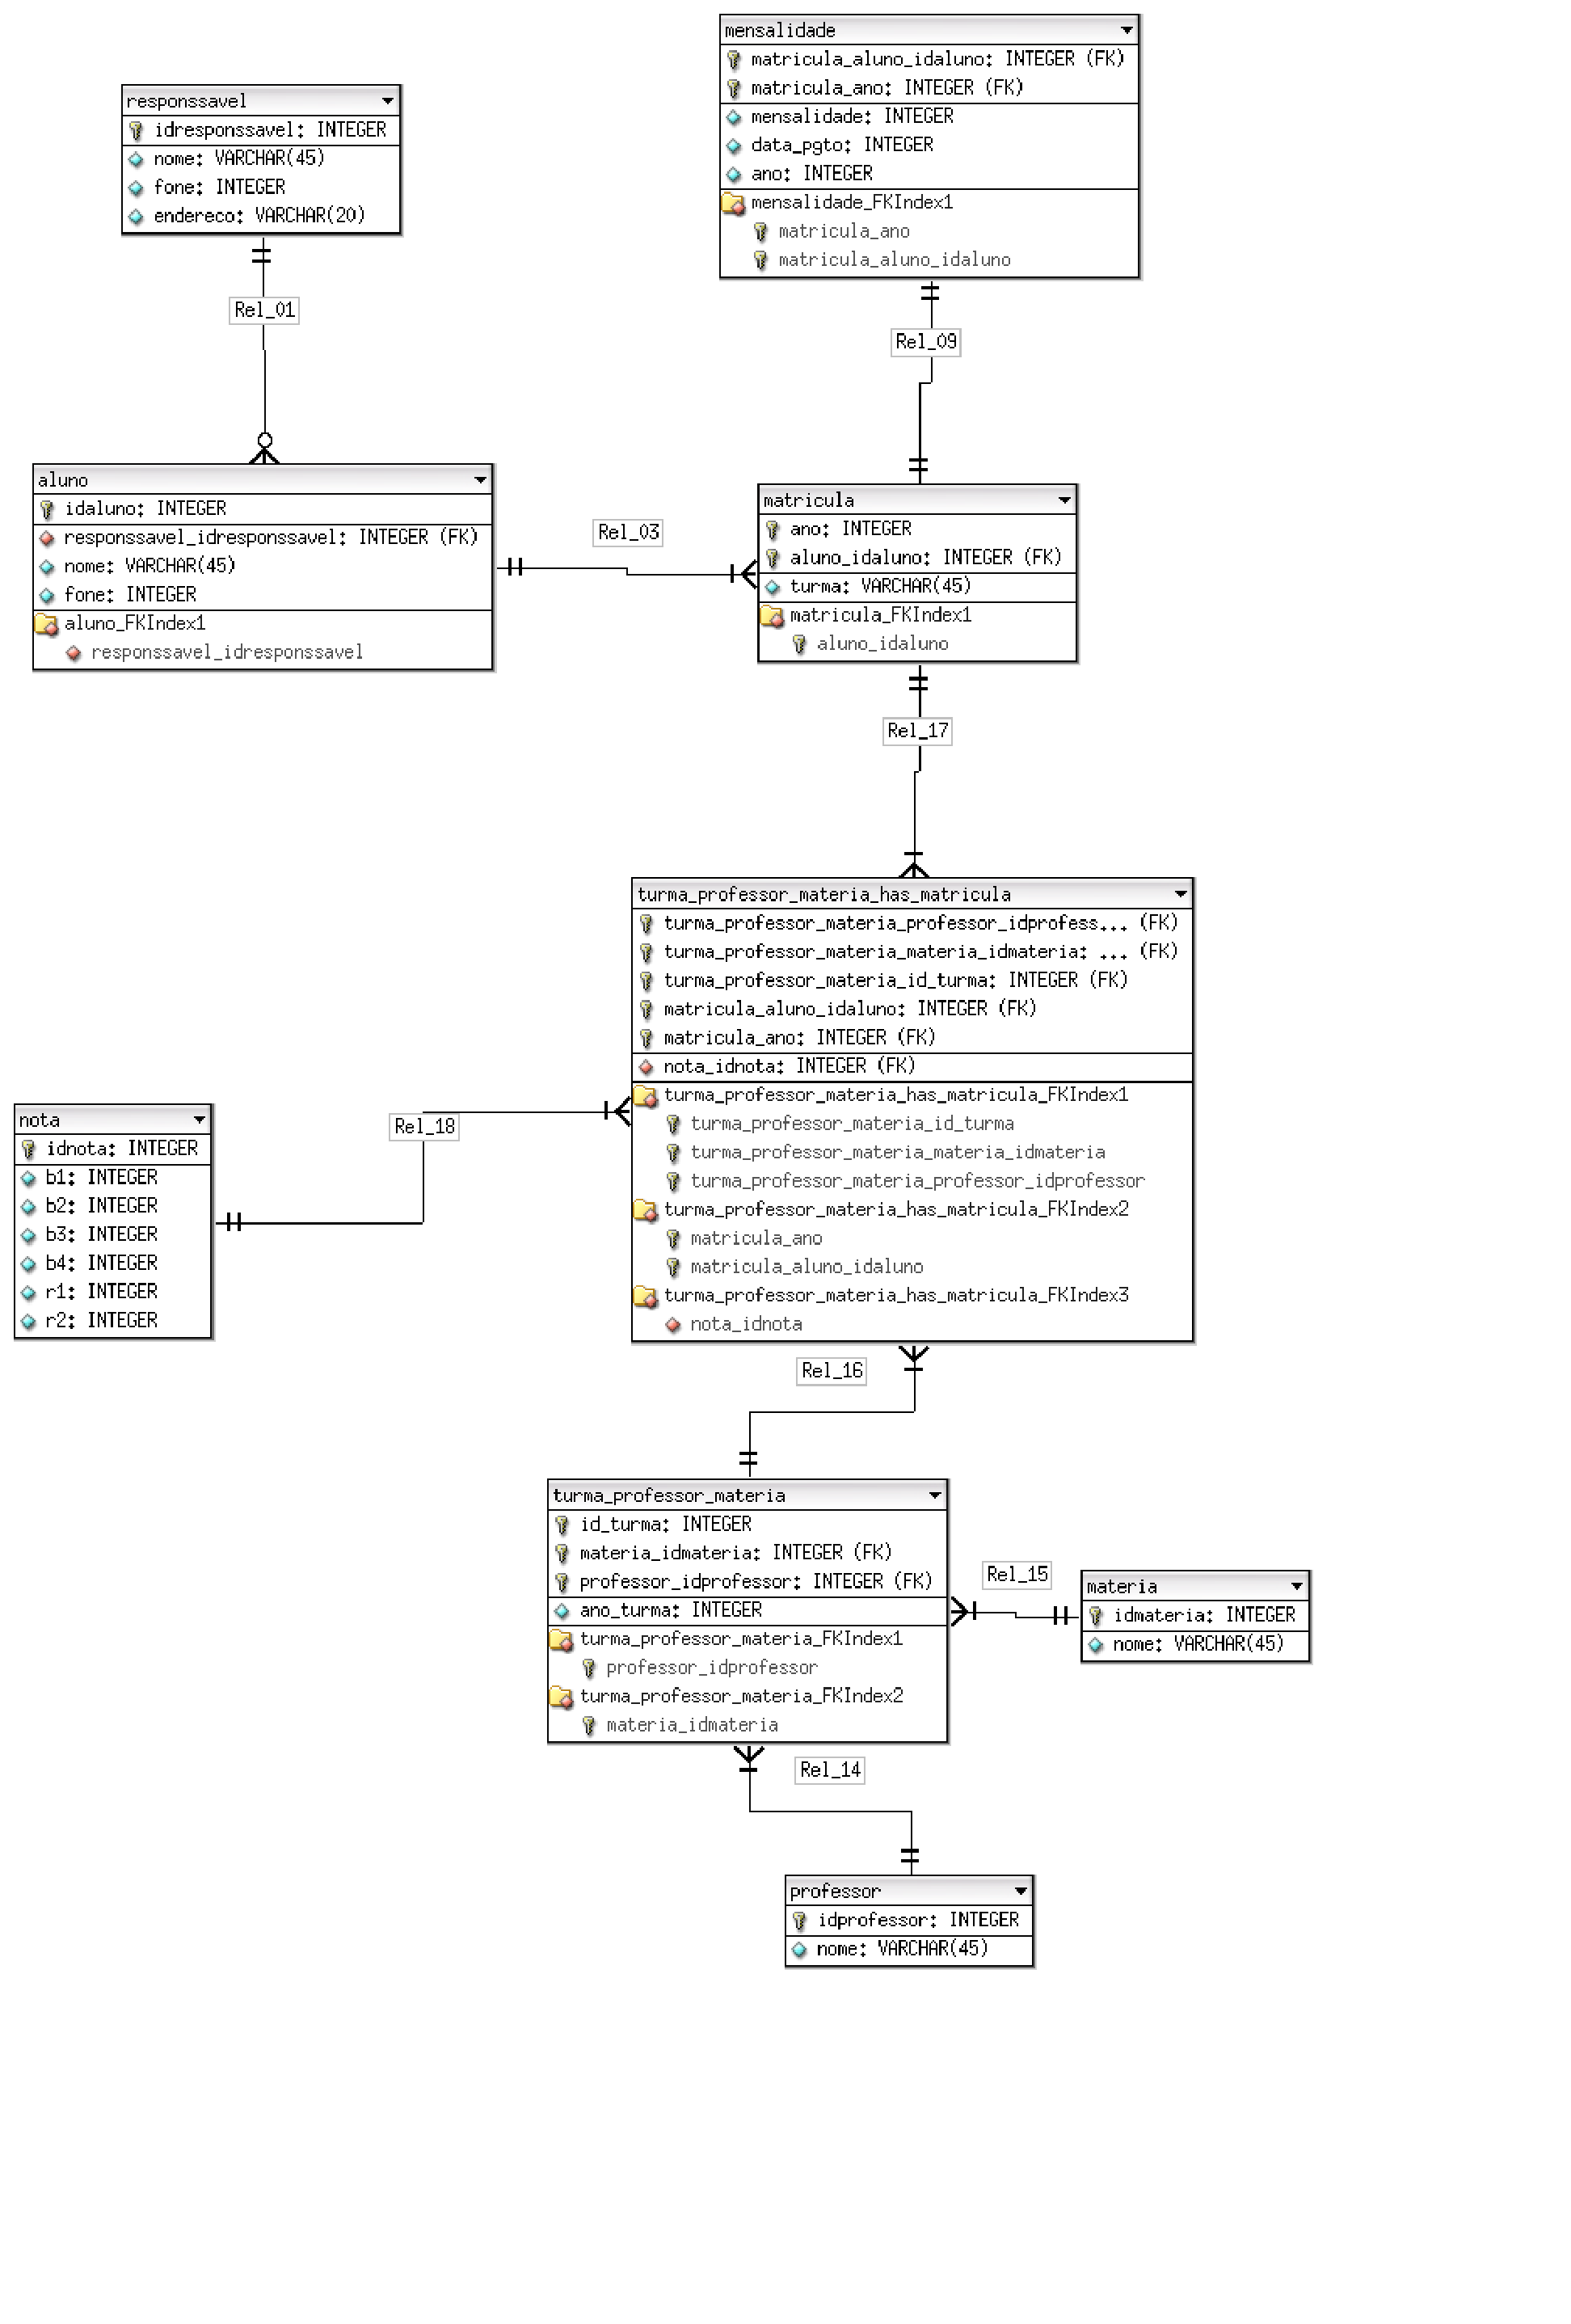
\includegraphics[width=.75\textwidth]{Figures/db_sch}
    \caption{Esquem�tio Entidade-Relacionamento}
    \label{fig:db_schema}
\end{figure}

\subsection{Cria��o do Banco}
A cria��o do Banco de dados foi feita como orientado pelo professor da
disciplina nas aulas de laborat�rio a partir do esquema \ref{fig:db_schema}feito no software
\textbf{DB Designer}.
\lstinputlisting[language=SQL]{../db_designer/db_escola_workbench_ver.sql}

\subsection{Inser��o de Valores}
A inser��o de dados no Banco foi feita como orientado no enunciado da quest�o.

\subsubsection{Respons�veis}
\lstinputlisting[language=SQL]{../db_designer/responsaveis_insertion.sql}

\subsubsection{Alunos}
\lstinputlisting[language=SQL]{../db_designer/alunos_insertion.sql}

\subsubsection{Professores}
\lstinputlisting[language=SQL]{../db_designer/professor_insertion.sql}

\subsubsection{Mat�rias}
\lstinputlisting[language=SQL]{../db_designer/materia_insert.sql}

\subsubsection{Forma��o das Turmas}
\lstinputlisting[language=SQL]{../db_designer/turma_professor_materia_insert.sql}

\subsubsection{Matr�cula}
\lstinputlisting[language=SQL]{../db_designer/Matricula_insert.sql}

subsubsection{Notas}
\lstinputlisting[language=SQL]{../db_designer/notas_insert.sql}

\subsubsection{Mensalidade}
\lstinputlisting[language=SQL]{../db_designer/mensalidade_insert.sql}

\end{section}

%%% EOF %%%


% Implementa��o: Funcionamento do circuito -------------------------------------
\begin{section}{Implementa��o}
A  implementa��o do scripts foi realizada no software
\textbf{mysql-workbench} usando \textbf{localhost@root} como servidor.\\
As consultas foram feitas seguindo o que era requerido no enunciado da quest�o.

\lstinputlisting[language=SQL]{../db_designer/consultas_r1_r6.sql}

\end{section}
%%% EOF %%%


% An�lise e Simula��o: Modelsim ------------------------------------------------
\begin{section}{Resultados}

\subsection{Diagrama do Sistema}

\begin{figure}
    \centering
    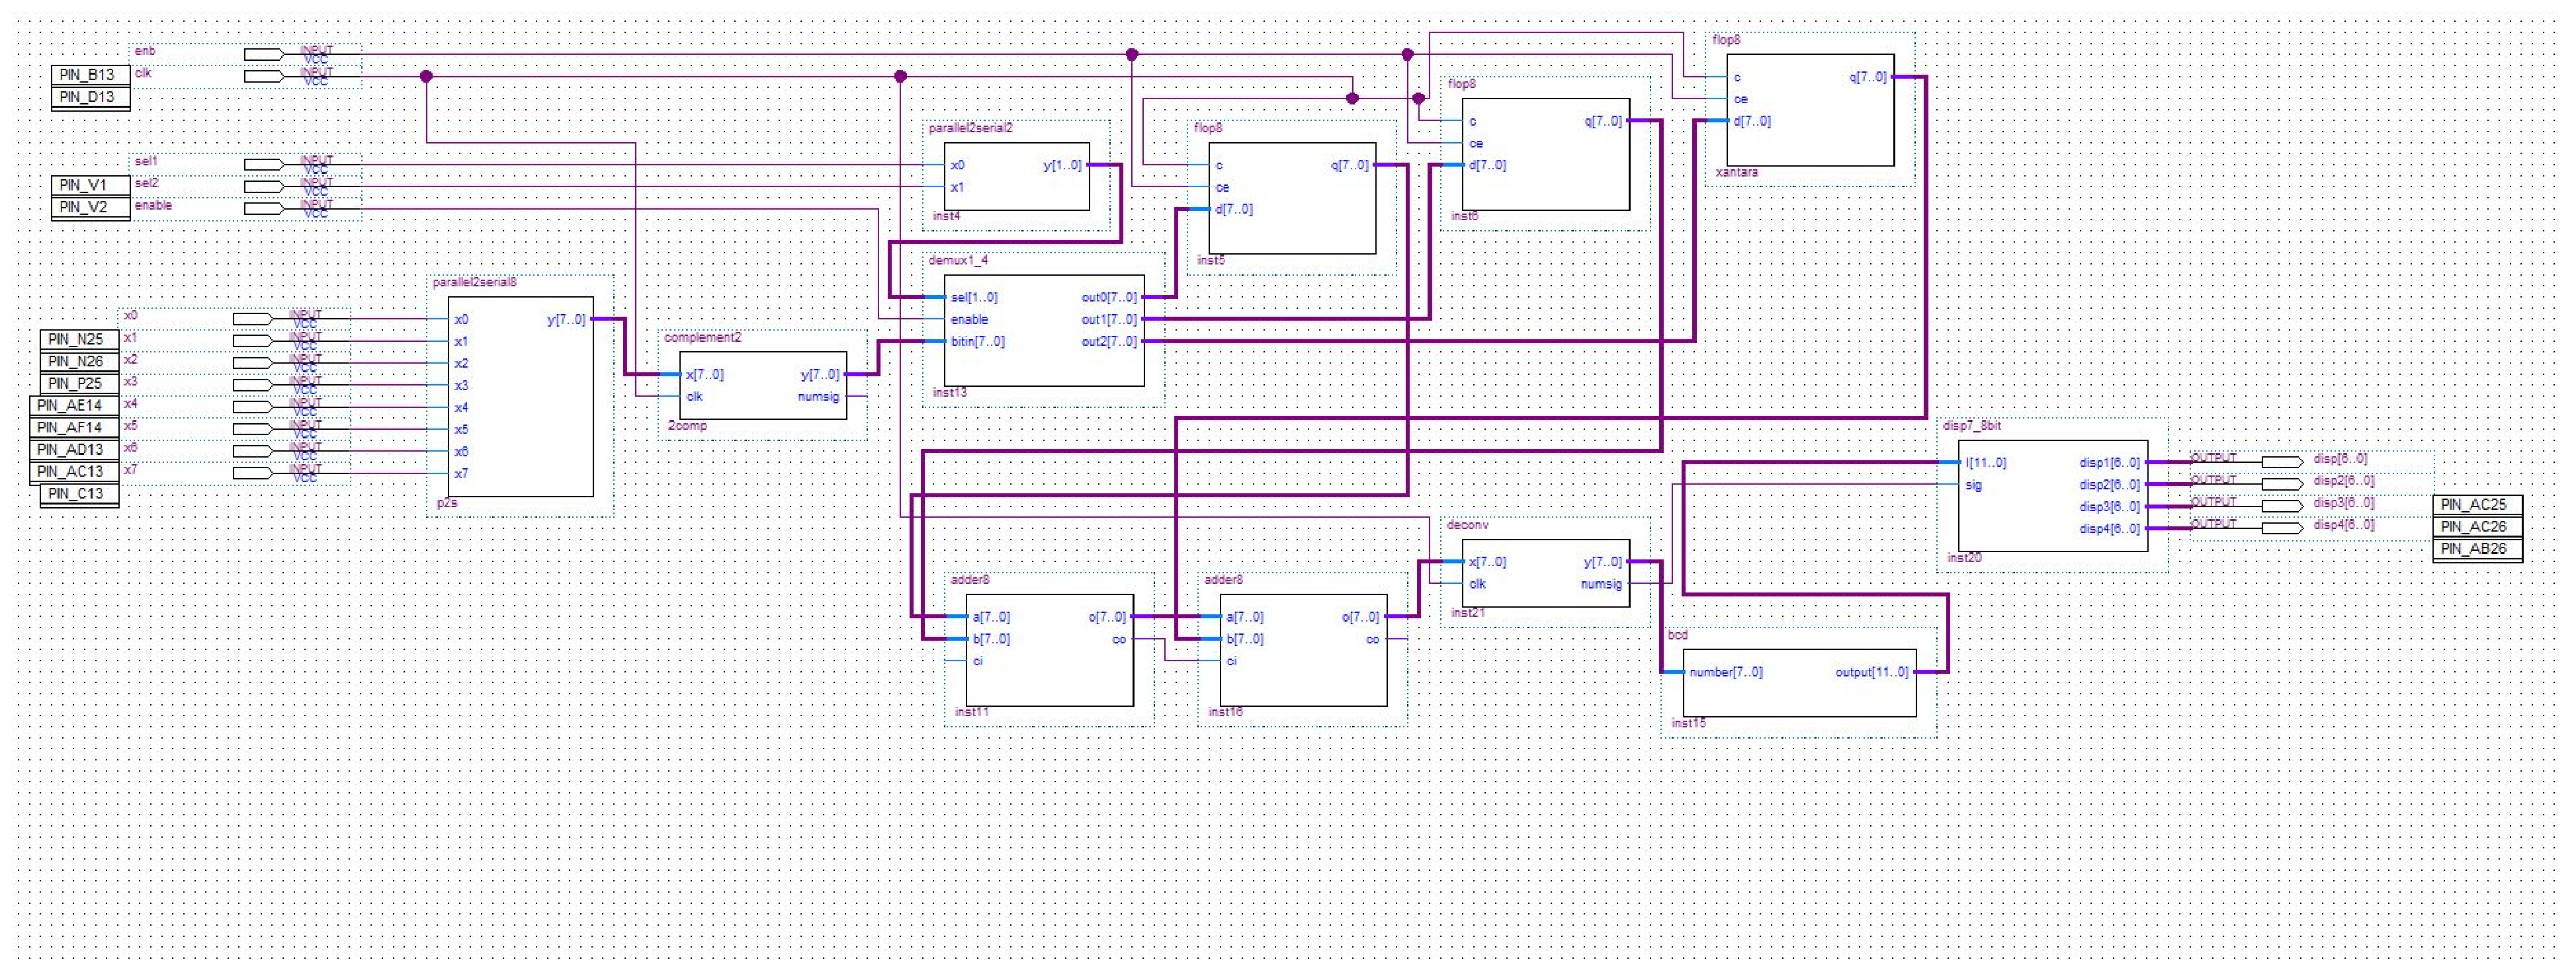
\includegraphics[width=.90\textwidth]{Figures/system_sch}
    \caption{Esquem�tico do Sistema no QuartusII}
    \label{fig:system}
\end{figure}

\subsection{Simula��o}
Todos os blocos do sistema foram devidamente simaulado sno \emph{ModelSim},
muitos por se tratarem de blocos intermedi�rios no sistema, n�o havia muito
sentido em algumas delas.\\
Abaixo � mostrada a sa�da da simula��o do bloco somador:

\begin{figure}
    \centering
    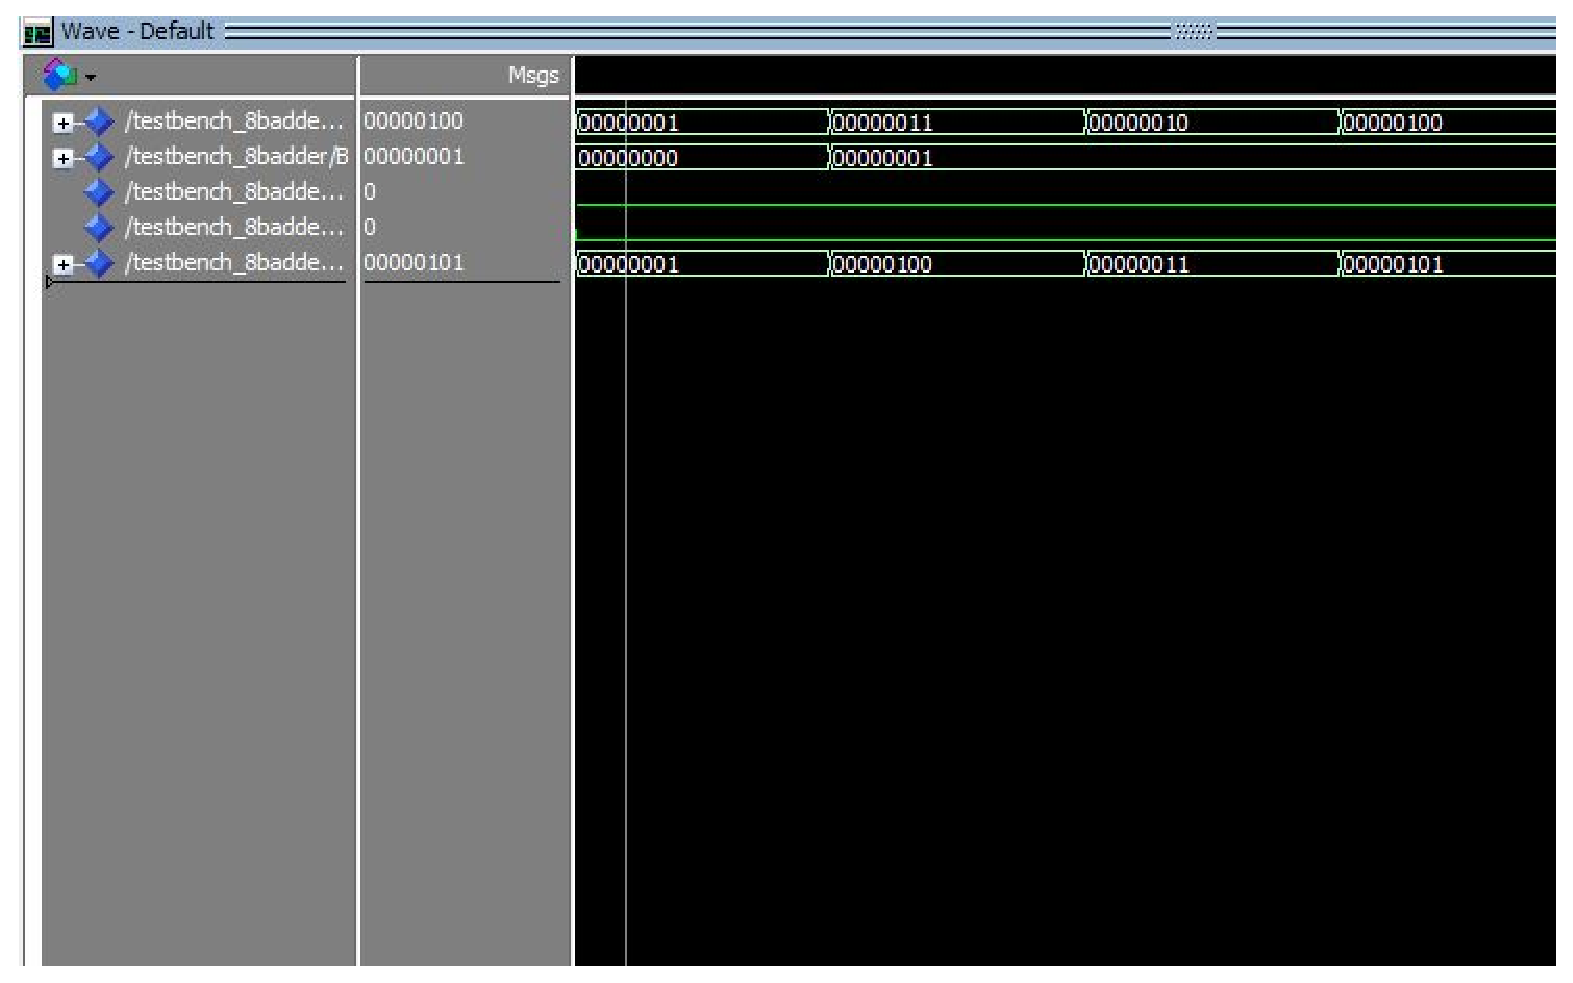
\includegraphics[width=.85\textwidth]{Figures/tb_adder8}
    \caption{Esquem�tico do Sistema no QuartusII}
    \label{fig:system}
\end{figure}

\subsection{Execu��o}
Na finaliza��o do projeto h� alguns pontos a serem salientados.\\

\begin{itemize}
    \item Durante o desenvolvimento do sistema houveram algumas diferen�as na simula��o e
no c�digo que foi mebarcado na fpga, ent�o a partir de certo ponto foi optado o
teste somente na placa.
    \item N�o houve tempo para tratamento de estouro de buffer, ent�o em alguns
        casos a sa�da era o resultado somado com um, o que foi resolvido
        retirando a liga��o entre carry in/carry out do primeiro para o segundo
        somador.
\end{itemize}

\end{section}
%%% EOF %%%


%\bibliographystyle{ieeetr}
%\bibliography{tech_report}

% C�digos e Background Matem�tico ----------------------------------------------
\newpage
\appendix
%\input{apendice}
\end{document}
%%% EOF %%%
